\begin{figure*}[]
\caption{DiffTrace Overview}
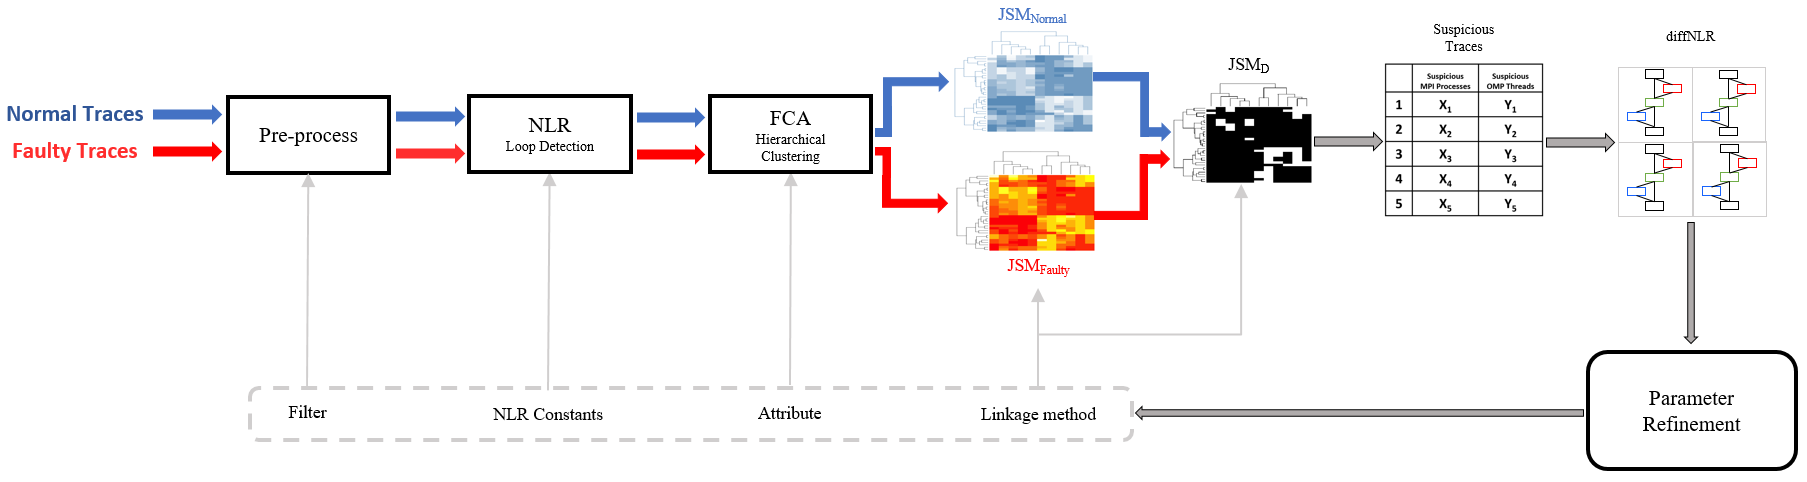
\includegraphics[width=0.95\textwidth]{figs/overview.png}
%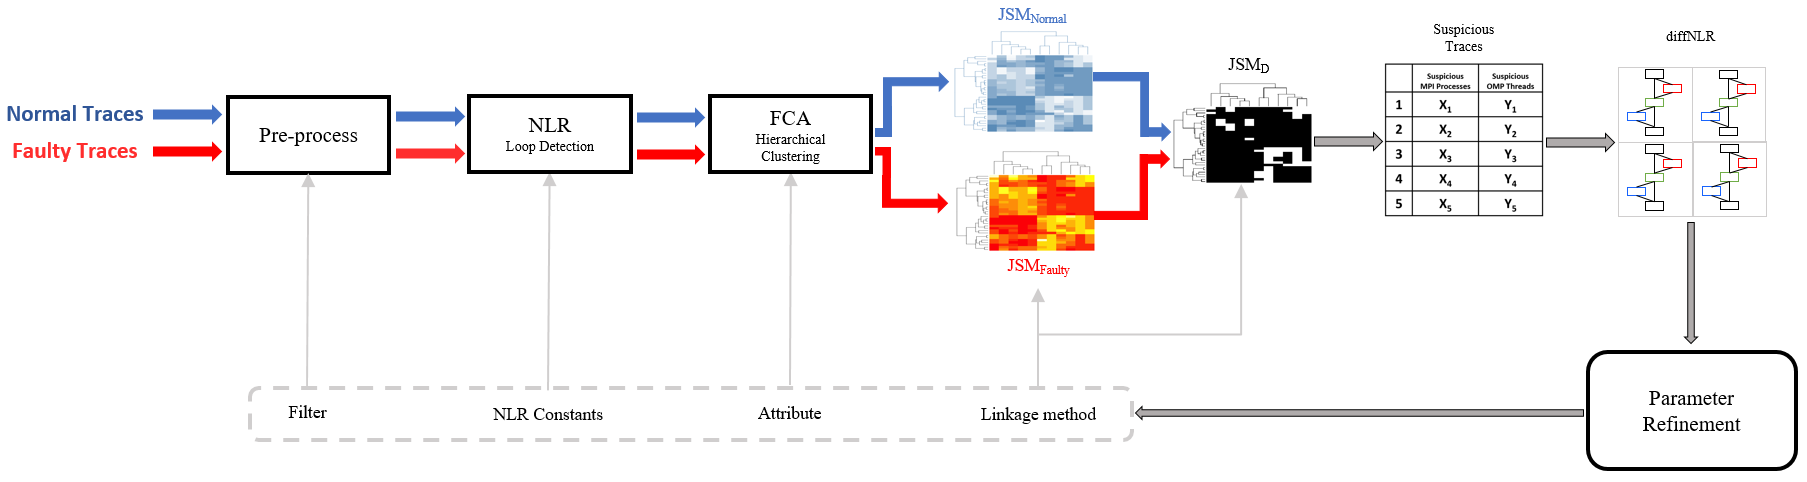
\includegraphics[]{figs/overview.png}
%\includegraphics[]{figs/overv}
\label{fig.diffTraceOverview}
\end{figure*}

The general idea is to utilize ParLOT \cite{ parlot} traces for studying HPC application behaviors towards fault detection and localization.
%
%ParLOT
ParLOT collects whole-program function calls and returns via dynamic binary instrumentation \cite{pin}, and incrementally compresses them on-the-fly.
%
ParLOT instruments and encodes functions within the binary to unique integers at two major levels: \textit{main image} only contains functions from the source-code and included APIs and \textit{all images} that cover system and library functions as well.
%
Upon termination of the application, ParLOT flushes out per-thread trace files each contains compressed sequence of executed function IDs.
%
The compression mechanism of ParLOT significantly reduces the time, memory and disk overhead, leaves the majority of the system bandwidth for the application. 
%

With the mindset of ``\textit{pay a little upfront to dramatically reduce the number of overall debug iterations}'', ParLOT well overcomes the challenge of whole-program \textit{trace collection} and leaves the \textit{trace analysis} for offline post-mortem analysis. 
%
However, raw ParLOT traces are just compressed sequences of executed function IDs per thread.
%
Also, enabling ParLOT on top of large-scale HPC applications execution would result in thousands of often-long traces.
%
The collected traces require to  get prepared, grouped and transformed to meaningful representations that reveal facts about the dynamic behavior of the program.

In this paper, we introduce DiffTrace, a tool-chain (figure \ref{fig.diffTraceOverview}) that provides infrastructures for \textit{iterative and configurable trace search space reduction towards localizing the fault} in a set of faulty traces.
%
Considering a ``successful’’ termination of the application as \textit{normal behavior}, DiffTrace iteratively compares the faulty traces against normal traces to detect any \textit{abnormal behavior}.
%
Each abnormal behavior is a potential fault cause or manifestation.
%
However, faults in HPC applications may occur or influence the program behavior at different locations and granularities, due to the often high and hybrid level of parallelism.
%
Also, typical HPC applications spend most of their execution time in a main loop until convergence or over time-steps.
%
A fault may get triggered at some point at the code and reflects itself right away, or after some progress from triggered point. 
%
Given a set of normal traces and faulty traces, DiffTrace feeds both sets into a sequence of data transformation and classification. Then suggests a few traces for deeper study (e.g., comparing actual traces from a specific vantage point) by \textit{measuring and locating points of differences}.
%
Since each DiffTrace components have multiple parameters and constants, evidences about what went wrong that made the program fails should get obtained \textit{iteratively}. In each iteration, by picking semantically well-tuned parameters, DiffTrace can put a flash-light on a specific aspect of the program dynamic behavior.
%

\begin{figure}[]
\centering
\caption{Simplified MPI implementation of Odd/Even Sort}
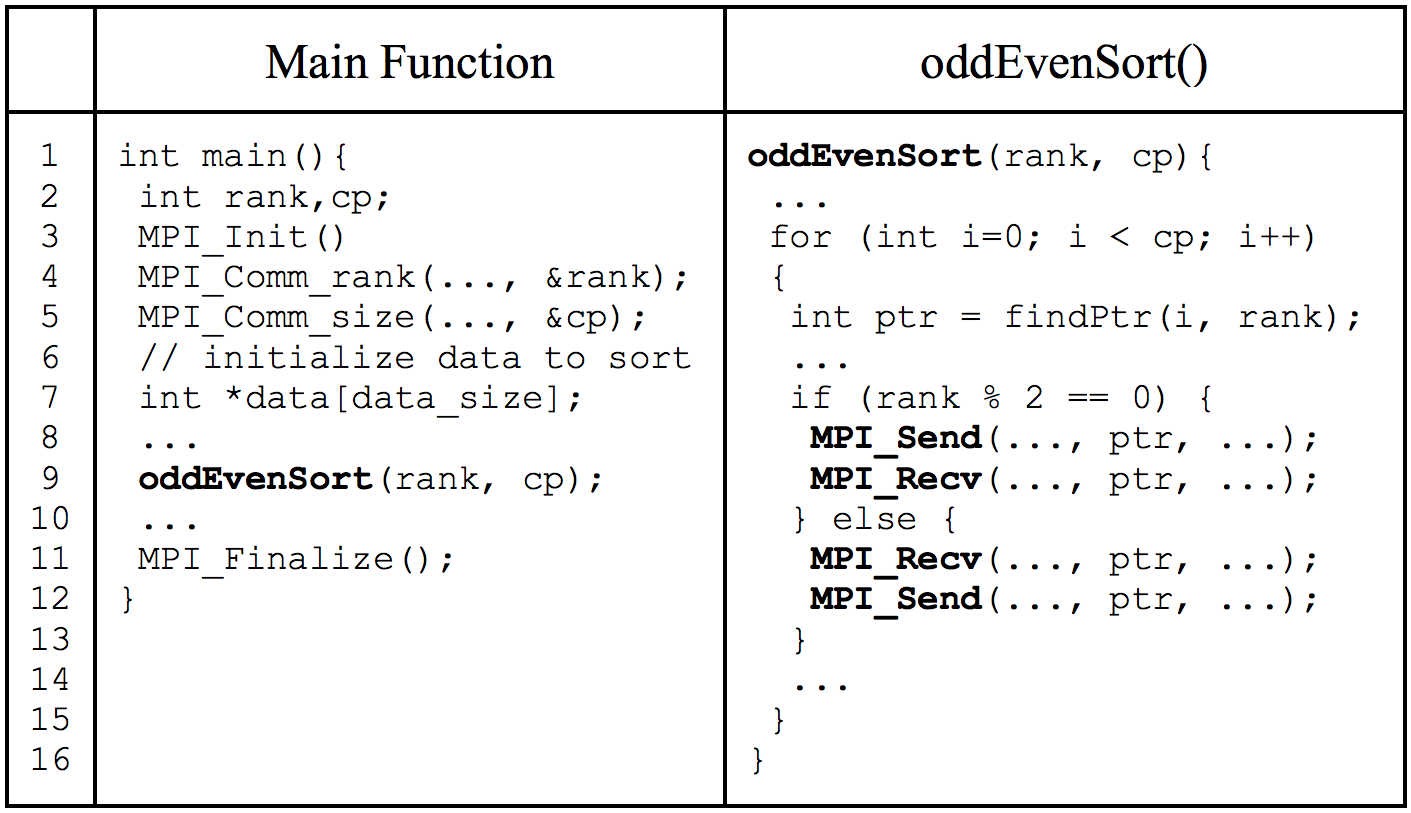
\includegraphics[width=0.45\textwidth]{figs/oddEven.png}
\label{fig.oddEven}
\end{figure}

The work-flow of DiffTrace starts with \textit{pre-processing} traces. ParLOT traces are highly compressed and often contain functions that might not be interesting from a certain point of analysis. DiffTrace decompresses and prunes traces, providing ``finer'' traces for later phases.  
%
Loops in source codes reflect themselves as a sequence of \textit{repetitive patterns}, resulting in often-long but redundant trace entries. A ``nested loop  recognition'' mechanism then mines loops from traces as ``\textit{a measure of progress}'' per thread, and also a loss-less abstraction to ease the rest of trace analysis.
%
The control flow of events in parallel architectures often follow a \textit{regular pattern} such as SPMD, odd-even and master/slave. This characteristic often makes all traces of a single execution tend to fall into just \textit{a few} ``conceptually equivalent classes''. 
%
%Adapted from the work by Webber et al \cite{weberStructural}, we have applied \textit{formal concept analysis} (FCA)\cite{clbook} techniques to reduce the trace search space into a few classes of traces, and also using the \textit{concept lattice} (CL) data structure as the \textit{model} of execution for further analysis.
%
\hl{definition of ``fault'' maybe? a software bug, node failure, a library version update or porting to a new system that cause failure to a working software }
To study the impact of a fault on a normal execution, DiffTrace classify collected traces and measures the \textit{similarity} between the equivalent classes of faulty execution against the corresponding fault-free execution.
%
The basic idea is to find out which traces (and consequently processes/threads) are falling into a different class (i.e., cluster) when the fault is introduced.
%
Based on the observed similarity of two clusterings, DiffTrace suggests top suspicious traces that are suffering the most from the fault for deeper analysis.
%

The rest of this section illustrates DiffTrace components on sets of ParLOT traces collected from MPI odd/even sort example(figure \ref{fig.oddEven}).
Odd/Even sort is a variant of the bubble-sort operates in two alternate phases: \textit{Phase-even} where even processes exchange (compare and swap) values with right neighbors and \textit{Phase-odd} where odd processes exchange values with right neighbors. The for loop in line 4 of \texttt{oddEvenSort()} iterates over phases of the algorithm and based on the phase, the appropriate partner for each rank is getting discovered by the function \texttt{findPtr()} (line 6). The odd/even ranks then exchange their chunks of data (lines 9-13) and a set of sort, merge and copy operations would be performed on received data by each rank (which are replaced by \texttt{...} in line 15 for simplicity).

According to MPI Standard , MPI\_Send is a \textit{blocking send} used the \textit{standard} communication mode in which MPI \textit{may} buffer outgoing messages and the send call may complete before a matching receive is invoked. On the other hand, buffer space may be unavailable, or MPI may choose not to buffer outgoing messages, for performance reasons. In this case, the send call will not complete until a matching receive has been posted, and the data has been moved to the receiver. So based on the MPI implementation, a swap of order in line 11-12 of figure \ref{fig.oddEvenDL} code might end up causing a deadlock. This section ends with showing that DiffTrace can extract evidences from traces to justify and locate the cause of such deadlocks and other faults. Later in the paper, we evaluate Difftrace on a real world hybrid MPI+OpenMP example.

\subsection{Pre-processing}
% Please add the following required packages to your document preamble:
% \usepackage{multirow}
\begin{table}[]
\centering
\caption{Applicable filters to PT contents based on regular expressions}
\label{tab:filters}
\scalebox{0.65}{
\begin{tabular}{|c|c|l|}
\hline
\textbf{Category} & \textbf{Sub-Category} & \multicolumn{1}{c|}{\textbf{Description}} \\ \hline
\multirow{2}{*}{Primary} & Returns & Filter out all returns \\ \cline{2-3} 
 & PLT & \begin{tabular}[c]{@{}l@{}}Filter out the ".plt" function calls for external functions/procedures that \\ their address needs to be resolved dynamically from Procedure Linkage \\ Table (PLT)\end{tabular} \\ \hline
\multirow{4}{*}{MPI} & MPI All & Only keep functions that start with "MPI\_" \\ \cline{2-3} 
 & MPI Collectives & Only keep MPI collective calls (MPI\_Barrier, MPI\_Allreduce, etc) \\ \cline{2-3} 
 & MPI Send/Recv & Only keep MPI\_Send, MPI\_Isend, MPI\_Recv, MPI\_Irecv and MPI\_Wait \\ \cline{2-3} 
 & MPI Internal Library & Keep all inner MPI library calls \\ \hline
\multirow{3}{*}{OMP} & OMP All & Only keep OMP calls (starting with GOMP\_) \\ \cline{2-3} 
 & OMP Critical & Only keep OMP\_CRITICAL\_START and OMP\_CRITICAL\_END \\ \cline{2-3} 
 & OMP Mutex & Only keep OMP\_Mutex calls \\ \hline
\multirow{4}{*}{System} & Memory & Keep any memory related functions (memcpy, memchk, alloc, malloc, etc) \\ \cline{2-3} 
 & Network & Keep any network related functions (network, tcp, sched, etc) \\ \cline{2-3} 
 & Poll & Keep any poll related functions (poll, yield, sched, etc) \\ \cline{2-3} 
 & String & Keep any string related functions (strlen, strcpy, etc) \\ \hline
\multirow{2}{*}{Advanced} & Custom & Any regular expression can be captured \\ \cline{2-3} 
 & Everything & Does not filter anything \\ \hline
\end{tabular}}
\end{table}
Using ParLOT decoder, each trace needs to get decompressed for further analysis.
Supporting the iterative approach of DiffTrace, corresponding function names of each function ID in traces are checked with some pre-defined (table \ref{tab:filters}) or custom regular expressions (i.e., \textit{filters}). In case of a match, DiffTrace would keep that function ID for later phases, otherwise that function ID would not be stored in the current iteration of DiffTrace.

Table \ref{tab:oddEvenPT} shows pre-processed traces ($T_i$) of odd/even sort execution with 4 processes. $T_i$ is the trace that stores function calls of process $i$.

\begin{table}[]
\centering
\caption{The generated PTs for odd/even execution with four processes}
\label{tab:oddEvenPT}
\scalebox{0.75}{
\begin{tabular}{|l|l|l|l|}
\hline
\rowcolor[HTML]{EFEFEF} 
\multicolumn{1}{|c|}{\cellcolor[HTML]{EFEFEF}\textbf{$PT_0$}} & \multicolumn{1}{c|}{\cellcolor[HTML]{EFEFEF}\textbf{$PT_1$}} & \multicolumn{1}{c|}{\cellcolor[HTML]{EFEFEF}\textbf{$PT_2$}} & \multicolumn{1}{c|}{\cellcolor[HTML]{EFEFEF}\textbf{$PT_3$}} \\ \hline \hline
... & ... & ... & ... \\ \\[-1em]  \hline
main & main & main & main \\ \\[-1em]  \hline
MPI\_Init & MPI\_Init & MPI\_Init & MPI\_Init \\ \\[-1em]  \hline
MPI\_Comm\_Rank & MPI\_Comm\_Rank & MPI\_Comm\_Rank & MPI\_Comm\_Rank \\ \\[-1em]  \hline
MPI\_Comm\_Size & MPI\_Comm\_Size & MPI\_Comm\_Size & MPI\_Comm\_Size \\ \\[-1em]  \hline
... & ... & ... & ... \\ \\[-1em]  \hline
oddEvenSort & oddEvenSort & oddEvenSort & oddEvenSort \\ \\[-1em]  \hline
... & ... & ... & ... \\ \\[-1em] \hline
findPtr & findPtr & findPtr & findPtr \\ \hline
\rowcolor[HTML]{FFCCC9} 
{\color[HTML]{333333} MPI\_Send} & \cellcolor[HTML]{CBCEFB}{\color[HTML]{333333} MPI\_Recv} & {\color[HTML]{333333} MPI\_Send} & \cellcolor[HTML]{CBCEFB}{\color[HTML]{333333} MPI\_Recv} \\ \hline
\rowcolor[HTML]{FFCCC9} 
{\color[HTML]{333333} MPI\_Recv} & \cellcolor[HTML]{CBCEFB}{\color[HTML]{333333} MPI\_Send} & {\color[HTML]{333333} MPI\_Recv} & \cellcolor[HTML]{CBCEFB}{\color[HTML]{333333} MPI\_Send} \\ \hline
... & ... & ... & ... \\ \hline
findPtr & findPtr & findPtr & findPtr \\ \hline
\rowcolor[HTML]{FFCCC9} 
{\color[HTML]{333333} MPI\_Send} & \cellcolor[HTML]{CBCEFB}{\color[HTML]{333333} MPI\_Recv} & {\color[HTML]{333333} MPI\_Send} & \cellcolor[HTML]{CBCEFB}{\color[HTML]{333333} MPI\_Recv} \\ \hline
\rowcolor[HTML]{FFCCC9} 
{\color[HTML]{333333} MPI\_Recv} & \cellcolor[HTML]{CBCEFB}{\color[HTML]{333333} MPI\_Send} & {\color[HTML]{333333} MPI\_Recv} & \cellcolor[HTML]{CBCEFB}{\color[HTML]{333333} MPI\_Send} \\ \hline
... & ... & ... & ... \\ \hline
MPI\_Finalize & MPI\_Finalize & MPI\_Finalize & MPI\_Finalize \\ \hline
\end{tabular}}
\end{table}



\subsection{Nested Loop Representation}
HPC applications often spend most of their times in \textit{loops}. Function calls within each loop body reflect themselves as \textit{repetitive patterns} in ParLOT traces. Inspired by ideas from detection of repetitive patterns in strings \cite{nakamura_fast_2013} and other data structures\cite{kmr}, we have adapted the Nested Loop Recognition (NLR) algorithm from Ketterlin et al\cite{Ketterlin-nlr} to detect repetitive patterns in ParLOT traces (more details in section \ref{subsec:algo-nlr}). Detecting such patterns ``measures progress'' per trace and reflects the delayed or unfinished/broken loops that potentially caused by a fault.

For example, the loop in line 3 of \texttt{oddEvenSort()} (figure \ref{fig.oddEven}) iterates 4 times in execution with 4 processes. Thus each $T_i$ contains 4 consecutive occurrence of either \texttt{MPI\_Send() - MPI\_Recv()} (even $T$s) or \texttt{MPI\_Recv() - MPI\_Send()} (odd $T$s). By keeping only MPI functions and converting each $T_i$ to its equivalent NLR (Nested Loop Representation), table \ref{tab:oddEvenPT} can be reduced to figure \ref{tab:oddEvenPT-r}. \textbf{L0} (pair of MPI\_Send - MPI\_Recv) and \textbf{L1} (pair of MPI\_Recv - MPI\_Send) are two main body loops that have been detected among pre-processed filters. Note that, since first and last processes have only one-way communication with their neighbors, $T_0$ and $T_3$ iterates over the loop half of other processes.

\hl{connect this section to next}

\begin{figure}[]
\centering
\caption{Trace NLRs}
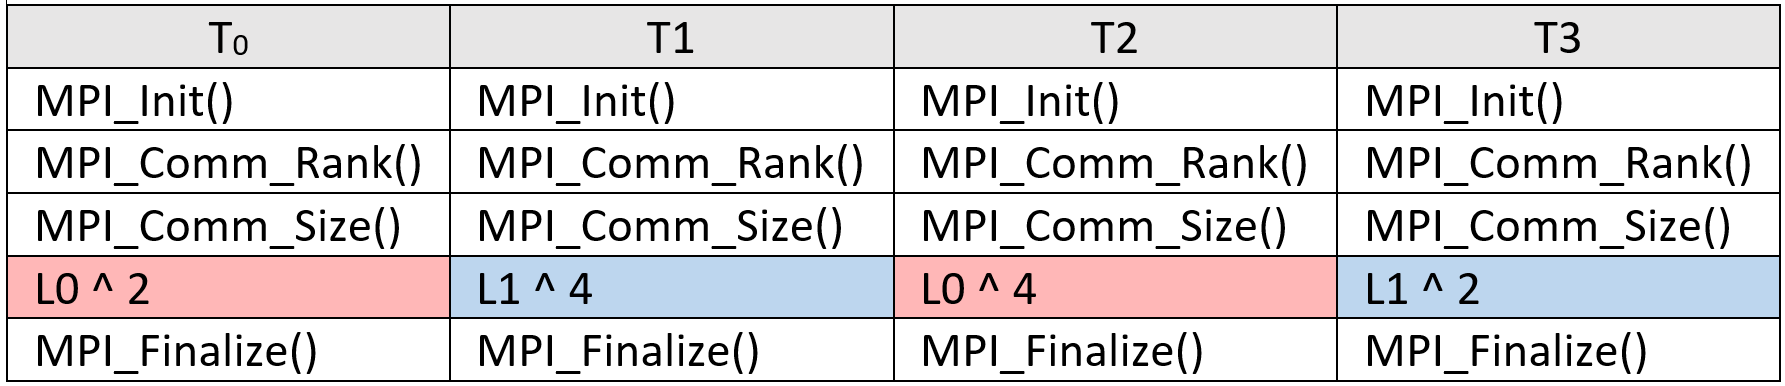
\includegraphics[width=0.45\textwidth]{figs/oddEvenPT-r.png}
\label{tab:oddEvenPT-r}
\end{figure}


\subsection{Hierarchical Clustering via FCA}
Underlying parallel software architecture of HPC applications often follow a \textit{regular pattern} with respect to sequences of executed functions. 
%
Considering this characteristic, per-thread individual function call traces can be classified into \textit{a few equivalent groups} based on the \textit{conceptual structure of trace contents}(i.e., sequence of functions).
% 
Such classification would distinguish naturally different threads (e.g., MPI processes from OpenMP threads in hybrid MPI+OpenMP applications), reduce the search space into just a few representative classes of traces and ease the process of detecting outlier traces.
%
In addition, the set of per-thread traces should be studied as ``a whole'' since there is a strong conceptual and causal relation among threads/processes.
%
In order to integrate all collected traces into a \textit{single model of execution} and forming ``equivalent classes of traces'', we have adapted the idea of \textit{Structural Clustering}  \cite{weberStructural} by applying \textit{formal concept analysis} (FCA)\cite{clbook} techniques to ParLOT traces.
%

A \textit{formal context} is a triple $K = (G, M, I)$, where $G$ is a set of \textbf{objects}, $M$ is a set of \textbf{attributes}, and $I \subseteq G \times M$ is an incidence relation that expresses \textit{which objects have which attributes}. Table \ref{tab:sampleContext}) shows the formal context of odd/even sort pre-processed traces. 

%
In this context, attributes are trace entries (function calls or detected loop bodies) without involving their frequency (e.g., loop counts). However, any set of attributes can be extracted from traces (table YY).
%
\hl{Definition of formal concept (needed?) figure }\ref{fig:formalConceptDefinition} :

\begin{figure}[]
\centering
\caption{Formal Concept Definition}
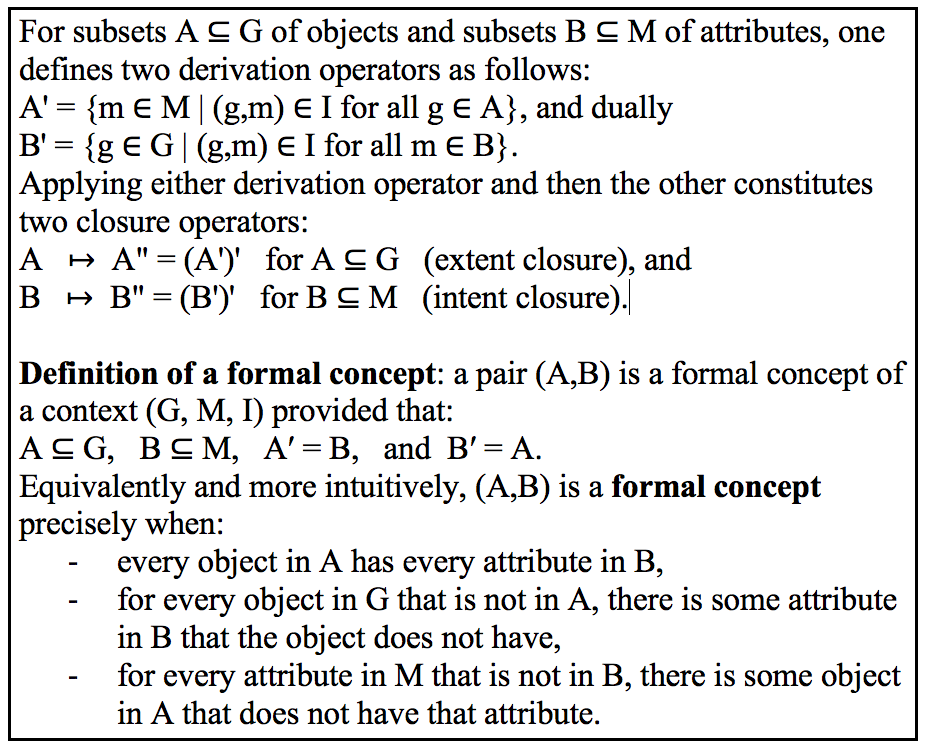
\includegraphics[width=0.45\textwidth]{figs/formalConceptDefinition.png}
\label{fig:formalConceptDefinition}
\end{figure}

A \textit{concept lattice} can be derived from a \textit{formal context} by specifying \textit{formal concepts} (figure \ref{fig:formalConceptDefinition}) and a \textit{partial order} on them. Concept lattices are represented as a directed acyclic graph where concepts are nodes and the order on them determines the edges.
%
Figure \ref{fig:sampleCL} shows the concept lattice of the formal context in 
%
The formal context in table \ref{tab:sampleContext} shows that all traces has the functions MPI\_Init(), MPI\_Comm\_size(), MPI\_Comm\_rank() and MPI\_Finalize(). Even traces have the loop \textit{L0} and odd traces have the loop \textit{L1}. The resulting concept lattice from this context is shown in figure \ref{fig:sampleCL} and reads as:

\begin{itemize}
	\item The top node indicates that all traces share MPI\_Init(), MPI\_Comm\_size(), MPI\_Comm\_rank() and MPI\_Finalize().
	\item The bottom node signifies that none of the traces share all attributes. 
	\item The middle nodes show that $T_0$ and $T_2$ are different from  $T_1$ and $T_3$
\end{itemize}

We have used concept lattices to obtain pair-wise \textit{similarity scores} among traces. The similarity metric that we have used is \textit{Jaccard Index}, also known as \textit{Intersection over Union}. For any pair of $(T_i,T_j)$, number of attributes in the Lowest Common Ancestor (LCA) node of $T_i$ and $T_j$ is the number of attributes that $T_i$ and $T_j$ have in common (intersection). The sum of the number of attributes of nodes in the path from each $T_i$ and $T_j$ to their LCA is the union. 
%
Figure \ref{fig:jsm2} shows the heatmap of full pair-wise Jaccard Similarity Matrix (JSM) obtained from the concept lattice in figure \ref{fig:sampleCL}.
%
DiffTrace uses obtained JSMs as \textit{linkage} function to form equivalent classes of traces by hierarchical clustering.
%
In the next phase of DiffTrace, we show how the differences of two hierarchical clustering from two executions (faulty vs. normal) can reveal which traces has been changed the most by the fault.




\begin{table}[]
\label{tab:sampleContext}
\caption{Context}
\scalebox{0.6}{
\begin{tabular}{l|cccccc}
 & \multicolumn{1}{l}{MPI\_Init()} & \multicolumn{1}{l}{MPI\_Comm\_Size()} & \multicolumn{1}{l}{MPI\_Comm\_Rank()} & \multicolumn{1}{l}{MPI\_Send()} & \multicolumn{1}{l}{MPI\_Recv()} & \multicolumn{1}{l}{MPI\_Finalize()} \\ \hline
Rank 0 & $\times$ & $\times$ & $\times$ &  & $\times$ & $\times$ \\
Rank 1 & $\times$ & $\times$ & $\times$ & $\times$ &  & $\times$ \\
Rank 2 & $\times$ & $\times$ & $\times$ & $\times$ &  & $\times$ \\
Rank 3 & $\times$ & $\times$ & $\times$ & $\times$ &  & $\times$
\end{tabular}}
\end{table}


\begin{figure}[t]
\centering
\scalebox{0.5}{
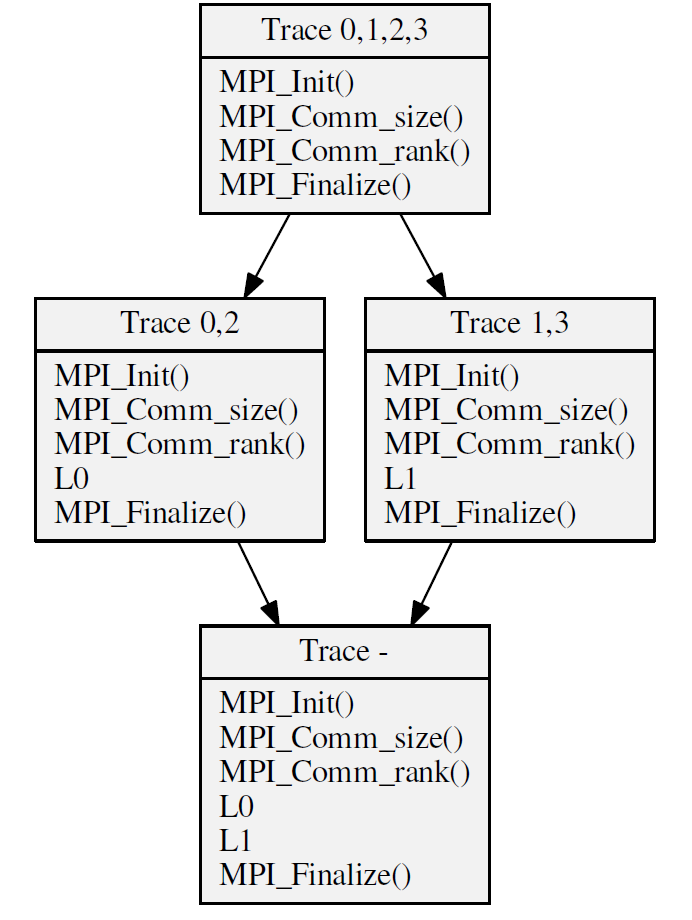
\includegraphics[width=3.4in]{figs/sampleCL.png}}
\caption{Sample Concept Lattice from Obj-Atr Context in table\ref{tab:sampleContext}}
\label{fig:sampleCL}
\end{figure}


%\begin{figure}[]
%\centering
%\scalebox{0.8}{
%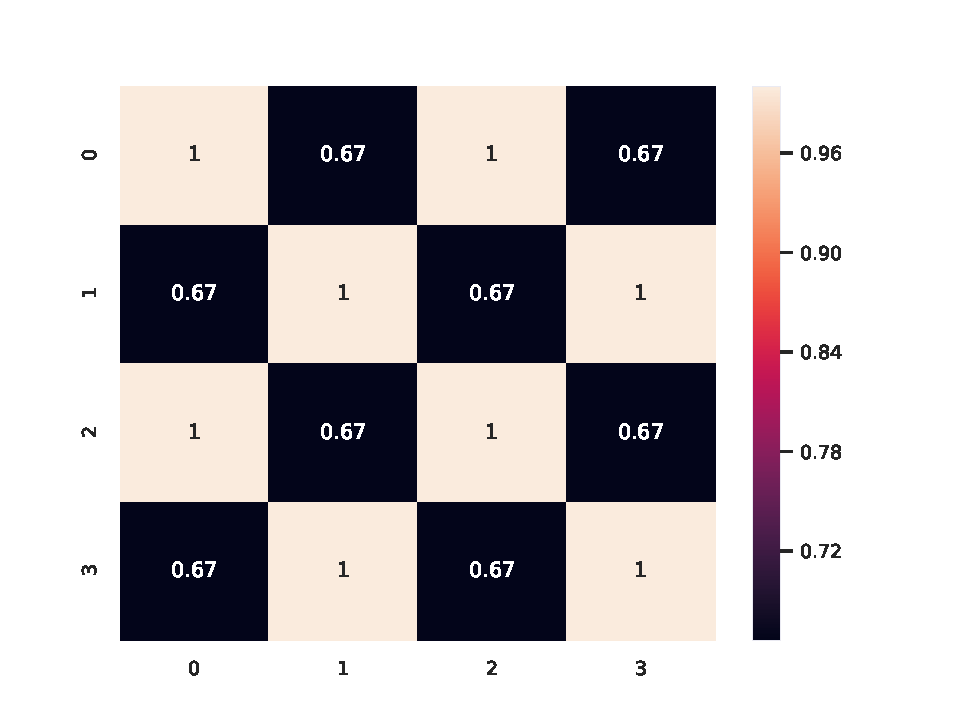
\includegraphics[width=3.4in]{figs/oddEvenJSM.pdf}}
%\caption{Pair-wise Jaccard Similarity Matrix (JSM) of MPI processes in Sample code}
%\label{fig:jsm}
%\end{figure}

\begin{figure}[]
\centering
\scalebox{0.8}{
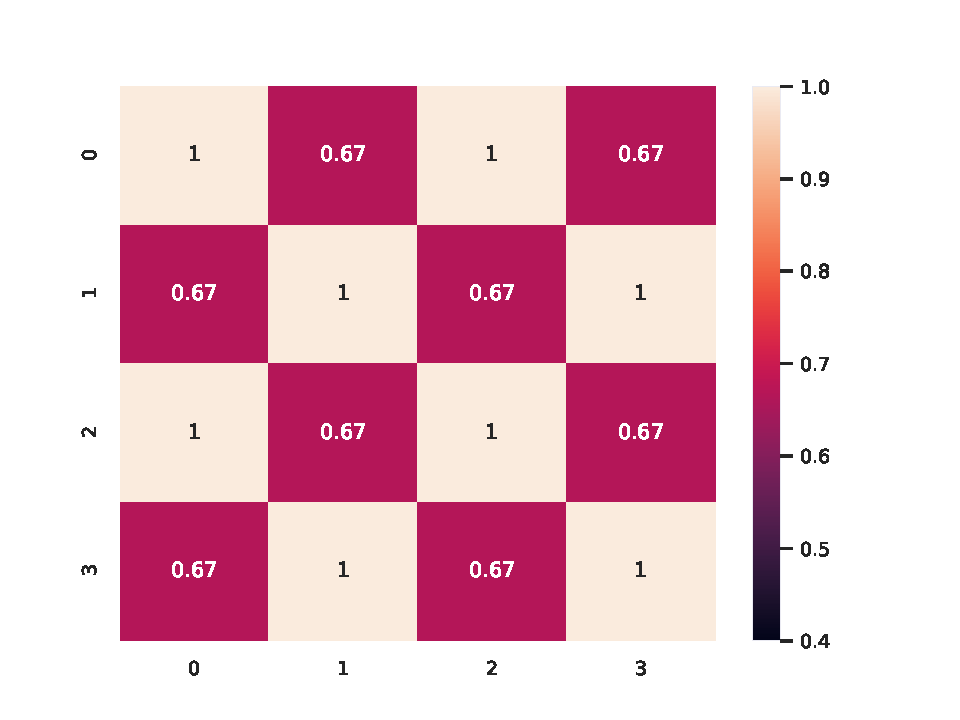
\includegraphics[width=3.4in]{figs/oddEvenJSM2.pdf}}
\caption{Pair-wise Jaccard Similarity Matrix (JSM) of MPI processes in Sample code}
\label{fig:jsm2}
\end{figure}


\subsection{Detecting Suspicious Traces via DiffJSM}
Up to this point, DiffTrace can narrow down the search space from numerous long traces to their equivalent JSM (i.e., clusters).
%
As the original intention of DiffTrace implies, we are interested in detecting what has changed the most when a fault is introduced with respect to the ``natural asymmetry'' of the application.
%
In other words, DiffTrace abstracts function call traces into JSMs which are reflections of asymmetry among traces. Now the hierarchical clustering based on the \textit{DiffJSM}, the subtraction of the faulty JSM from its corresponding normal JSM, would put the trace(s) that changed the most in a separate cluster from the others (i.e., outlier).
% 
The obtained outlier traces are candidates of the potential cause of the change in the program behavior, thus a potential fault root cause or fault manifestation.
%
However, a single iteration of DiffTrace (with a single set of parameters shown as dotted box in figure \ref{fig.diffTraceOverview}) might not reflect such asymmetries in the normal and faulty traces. 
%
Also different set of parameters might produce inaccurate suggestions (false positives).
%
To improve the accuracy of suggested suspicious traces (ranking table), we have sorted the suggestion table based on the \textit{B-score} similarity metric of two hierarchical clustering \cite{fowlkes83}. (more in section 3.B-score).

To evaluate the effectiveness of DiffJSM idea on suggesting suspicious traces, we have planted two artificial bugs (\textit{swapBug} and \textit{dlBug}) in the code in figure \ref{fig.oddEven} and launched the code with 16 processes. 
%
\textit{swapBug} swaps the order of MPI\_Send and MPI\_Recv in rank 5 after 7th iteration (of the loop in line 3 of \texttt{oddEvenSort}) simulating a potential deadlock and \textit{dlBug} simulates an actual deadlock (e.g., infinite loop) in the same location (rank 5 after 7th iteration).
%
Upon collection of ParLOT traces from execution above buggy versions, DiffTrace first decompresses traces and filters out all non-MPI functions.
Then two major loops are detected, \textbf{L0} and \textbf{L1}  (figure \ref{fig.gdiffs}-(a)) that are supposed to occur 16 times in even and odd traces, respectively (except for first and last trace which is 8 times).
After constructing concept lattices and their corresponding JSMs, $T\prime=5$ has been suggested as the most probable trace that got affected by the artificial bugs.

\subsubsection{introducing diffNLR}
To show the actual points of differences in suspicious traces with their corresponding normal trace, DiffTrace visualizes the common and different blocks of a pair of pre-processed trace via \textit{diffNLR}, a graphical visualization of \texttt{diff} algorithm \cite{diff-myers}.
%
\texttt{diff} takes two sequences $S_A$ and $S_B$ and computes the minimal \textit{edit} to convert $S_A$ to $S_B$. This algorithm has been used in GNU \texttt{diff} to compare two text files and in git for efficiently keeping track of file changes.
Since ParLOT preserves the order of function calls in the binary, each per thread trace $T_i$ is totally ordered, thus \textit{diff} can reflect the differences of a pair of $T$s. \textit{diffNLR} aligns common and different blocks of a pair of sequences (e.g., traces) horizontally and vertically, making it easier for analyst to see the differences of a pair of sequences in a glance.  
For simplicity, our implementation of \textit{gdiff} only takes one argument $x$ as \textit{the suspicious trace}

\textit{gdiff}$(x) \equiv $ \textit{gdiff}$(T_x,T_x^\prime)$

where $T_x$ is the trace of thread/process $x$ of a normal/successful execution and $T^\prime_x$ is the corresponding trace of faulty execution.

Figure \ref{fig.gdiffs}-(b) shows the $diffNLR(5)$ of \textit{swapBug} where $T_5$ iterates over the loop [MPI\_Recv - MPI\_Send] for 16 times (L1\^{}16) after the MPI initilization while the order swap has well reflected in $T_5^\prime$ (L1\^{}7 - L0\^{}9). Both processes seem to be terminated fine by executing MPI\_Finalize(). 
However, $diffNLR(5)$ of \textit{dlBug} (figure \ref{fig.gdiffs}-(c)) shows that while $T_5$ have executed MPI\_Finalize and terminated well, $T_5^\prime$ got stuck after executing L1 seven times and have never reached MPI\_Finalize.

This example shows that our approach can locate the impacted part of each execution by a fault. Having a pre-understanding of \textit{how the application should behave normally} would reduce the number of iterations by picking the right set of parameters on each pass. 


\begin{figure}[]
\centering
\caption{A line change in oddEvenSort (left) that might cause a deadlock in oddEvenSort\_DL (right)}
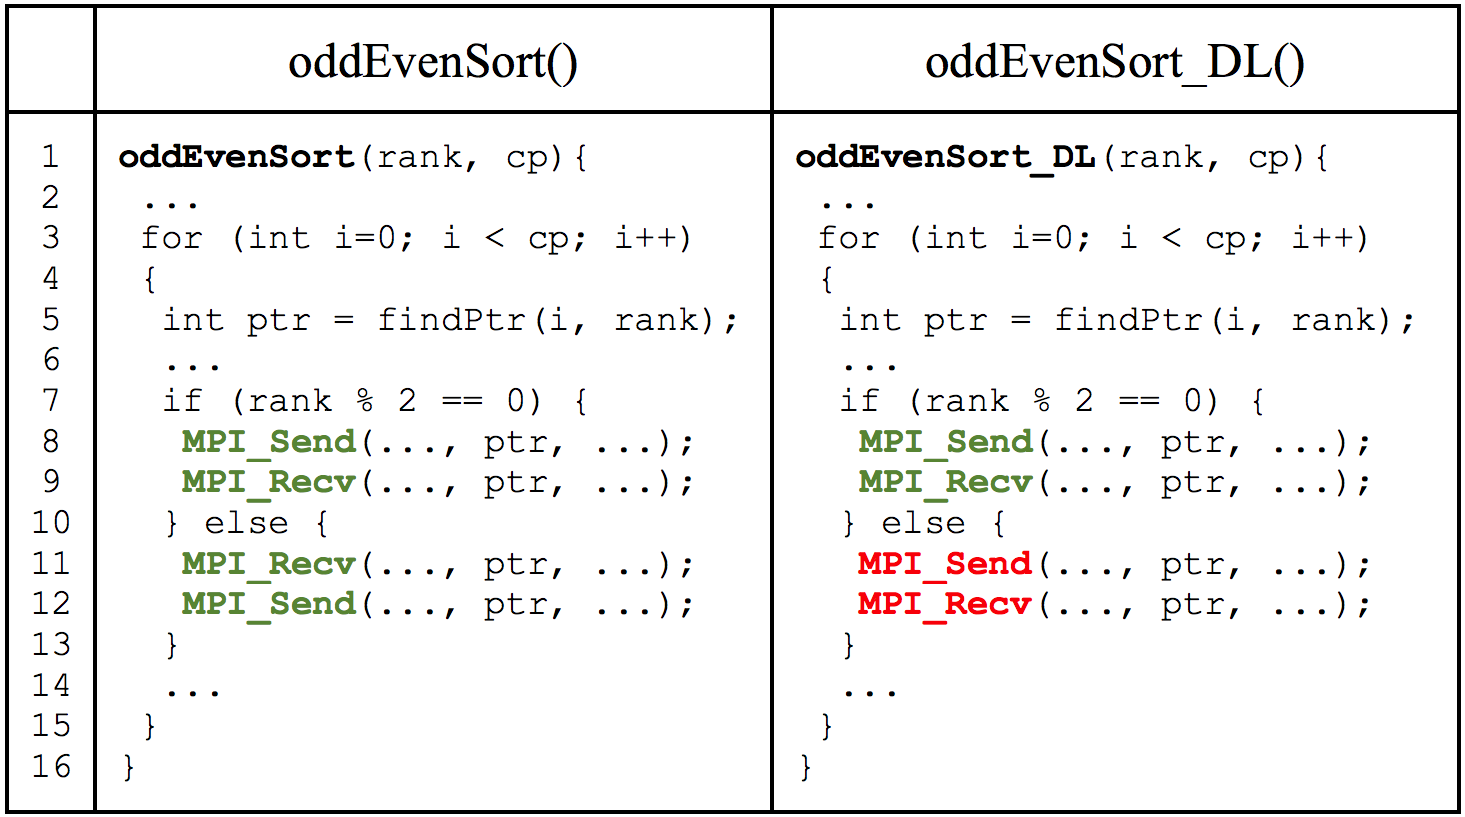
\includegraphics[width=0.45\textwidth]{figs/oddEvenDL.png}
\label{fig.oddEvenDL}
\end{figure}


\begin{figure}[]
\centering
\caption{(a) The legend of \textit{gdiff} and the list of loop structures (b) \textit{gdiff(5)} of \textit{swapBug} (c) \textit{gdiff(5)} of \textit{dlBug}}
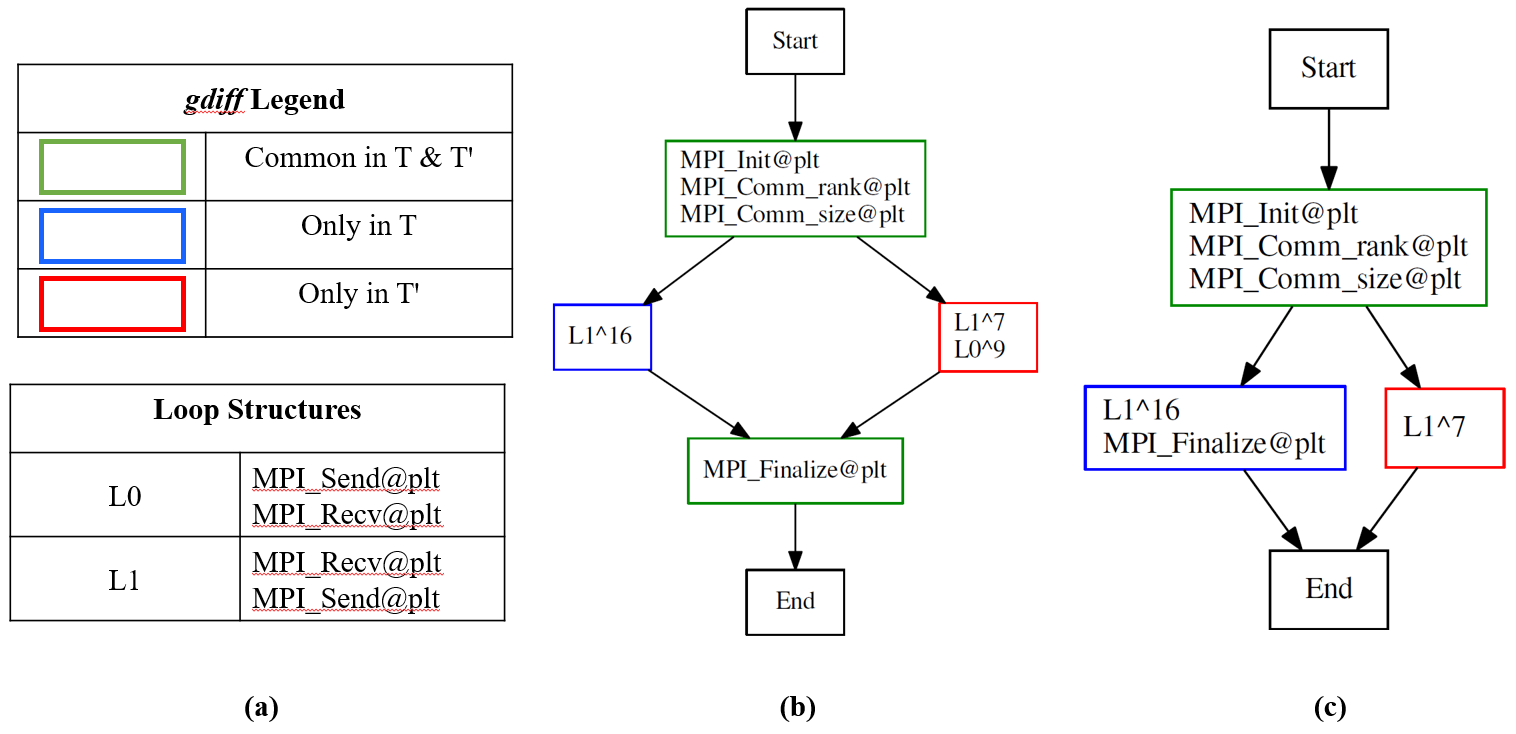
\includegraphics[width=0.45\textwidth]{figs/sampleGdiff.png}
\label{fig.gdiffs}
\end{figure}





%
%In the remainder of this section, we describe a chain of techniques that we apply to collected traces with having three main goals in mind:
%\begin{itemize}
%\item selectively pre-processing of traces to prune out uninteresting trace entries when we want to study a certain aspect of the dynamic behavior of the application. 
%\item reducing the search space by forming ``equivalent classes of traces'' and locating the trace or set of traces that got impacted the most by the fault.
%\item visualizing and reflecting the impact of fault to the potential faulty trace with respect to its corresponding fault-free trace.  
%\end{itemize}